
\chapter{Implementierung}

In diesem Kapitel wird auf Besonderheiten und Schwierigkeiten bei der Implementierung eingegangen.


%Weitestgehend wie in \autoref{draft:architecture}, aber Futures, tokio, Queues

\section{Continuous Integration mittels Jenkins}

Mittels der Continuous Integration Software Jenkins wird die Rust-Implementation nach jeder Aktualisierung der Quellcode-Repository gebaut.
In einem Jenkinsfile\footnote{Eigenname: \url{https://jenkins.io/doc/book/pipeline/jenkinsfile/}} ist hierzu die folgende Pipeline definiert:

\begin{figure}[H]
	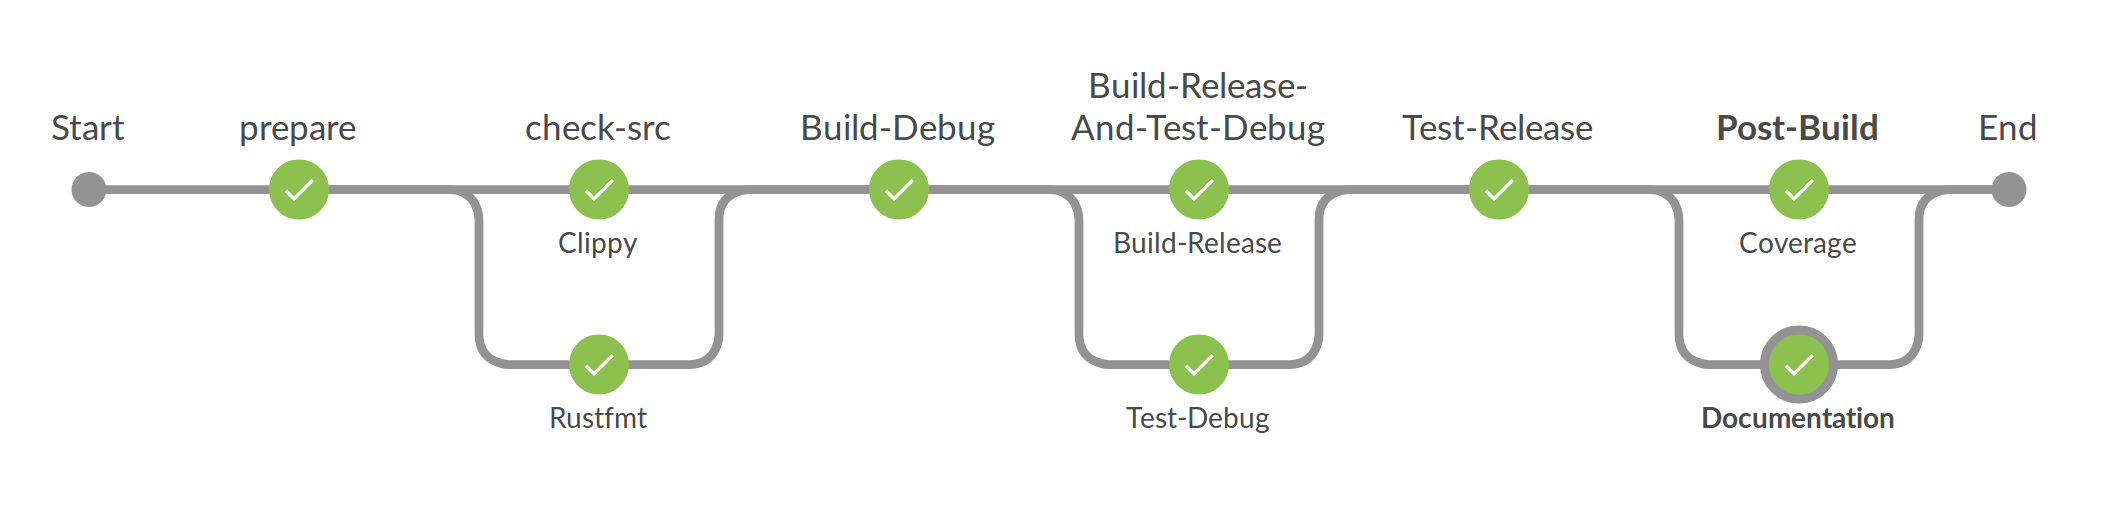
\includegraphics[width=\textwidth]{images/jenkins_pipeline_graph.png}
	\caption{Jenkins Pipeline Graph}
	\label{impl:jenkins:pipeline:graph}
\end{figure}

Im Folgenden sind die einzelnen Schritte genauer erklärt.


\subsubsection{Schritt \enquote{prepare}}
In diesem Schritt wird überprüft, ob die richtige Version von Rust installiert ist.
Sowohl der Rust Compiler als auch Abhängigkeiten wie Cargo, Clippy oder Tarpaulin werden falls nötig  in diesem Schritt nachinstalliert und aktualisiert.

\subsubsection{Schritt \enquote{check-src}}
Hier wird der Quellcode auf einen schlechten Programmierstil oder schlechte Programmierpraktiken durch Clippy und auf eine nicht standardkonforme Formatierung überprüft.
Ein erkannter Mangel resultiert in einen Abbruch und einem entsprechendem roten Icon auf der Projektseite auf Jenkins.
Ein Quellcode, der diese Qualitätsstandards nicht erfüllt, wird somit schnellstmöglich abgelehnt.

\subsubsection{Schritt \enquote{Build-Debug}}
In diesem Schritt wird das Projekt im Debug-Modus compiliert.
In einem Debug-Modus werden nahezu keine Optimierungen durchgeführt, weswegen die Ausführgeschwindigkeit meist mangelhaft ist.
Im Falle eines Fehlers in einem Unit-Test, können aus einem Debug-Artefakt jedoch nützlich Informationen gewonnen werden.

\subsubsection{Schritt \enquote{Build-Release-And-Test-Debug}}
Wie der Name bereits vermuten lässt, wird in diesem Schritt das Projekt im Release-Modus übersetzt.
Gleichzeitig wird das zuvor erstellte Debug-Artefakt auf Fehler überprüft, indem Unit-Tests ausgeführt werden.
Ein Release-Artefakt ist stark optimiert und ist für den Produktivbetrieb gedacht.

\subsubsection{Schritt \enquote{Test-Release}}
In diesem Schritt wird das Release-Artefakt mittels Unit-Tests auf Fehler überprüft.
Hierdurch soll sichergestellt werden, dass kein Fehler durch Optimierungen des Compilers aufgedeckt oder verursacht wurde.
Des weiteren soll kein Artefakt archiviert werden, das nicht auf Fehler überprüft wurde.

\subsubsection{Schritt \enquote{Post-Build}}
Dieser Schritt dient zur Zusammenstellung der Testabdeckung der Unit-Tests und der automatisierten  Erstellung der Dokumentation.

\subsubsection{Ergebnis des erfolgreichen Durchlaufs}
Jede Aktualisierung der Quellcoderepository resultiert bei erfolgreicher Compilation und Durchlaufen der Tests in den folgenden Artefakten:
\begin{itemize}
	\item \textbf{Debug-Artefakt}: Compilation für eine manuelle Fehlersuche mit vielen auf den Quellcode bezogenen Symbolen und ohne Optimierungen durch den Compiler
	\item \textbf{Release-Artefakt}: Kompilat mit Optimierungen für den Produktivbetrieb
	\item \textbf{Testbericht}: Bericht über wie viele Zeilen, Dateien, Klassen und Verzweigungen durch die Unit-Tests getestet wurden.
	\item \textbf{Dokumentation}: Die aus dem Quellcode generierte Dokumentation inklusive der Dokumentationen der Abhängigkeiten.
\end{itemize}

Für jeden erfolgreichen Bauvorgang, werden die erhobenen Informationen in die folgenden Graphen auf der Projektseite auf Jenkins übernommen:

\begin{figure}[H]
	\centering
	\begin{subfigure}{.5\textwidth}
		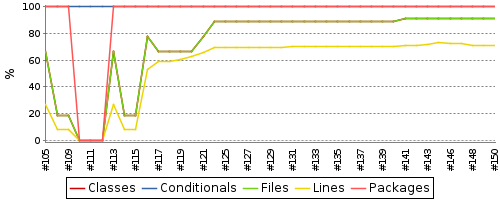
\includegraphics[width=\textwidth]{images/jenkins_coverage_graph.png}
		\caption{Jenkins Coverage Graph}
		\label{impl:jenkins:coverage:graph}
	\end{subfigure}%
	\begin{subfigure}{.5\textwidth}
		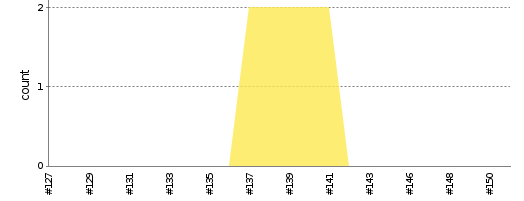
\includegraphics[width=\textwidth]{images/jenkins_warnings_graph.png}
		\caption{Jenkins Warnings Graph}
		\label{impl:jenkins:warnings:graph}
	\end{subfigure}
\end{figure}

\autoref{impl:jenkins:coverage:graph} zeigt die Testabdeckung seit Aufzeichnungsbeginn.
Die frühen und starken Schwankungen resultieren aus Testdurchläufen bei der Einrichtung des Graphen.
\autoref{impl:jenkins:warnings:graph} zeigt Warnungen, die der Rust Compiler für die verschiedenen Builds ausgegeben hat.

Die Graphen starten bei unterschiedlichen Versionen, da sie nacheinander eingerichtet wurden.

\clearpage
\section{Asynchrone Kommunikation}
Wie bereits in \autoref{design:communication:architecture:async} festgestellt, ist für eine hochperformante Kommunikationsplattform eine interne, asynchrone Kommunikation nötig.

\todo{Message Queuing Pattern \cite[207]{douglass2003real}}

Mittels \enquote{channel} (dt. \enquote{Kanäle}) können in Rust Mitteilungen zwischen vielen Auftraggebern und einem Empfänger ausgetauscht werden (andere Rust-Bibliotheken erlauben auch viele Empfänger, zum Beispiel \enquote{crossbeam-channel}\footnote{\url{https://crates.io/crates/crossbeam-channel}}).
Der zu versendende Datentyp muss lediglich das Merkmal \rustcinline{Send} aufweisen (siehe \autoref{rust:trait:send}):

\rustcinclude
	{impl:channels:example}
	{Beispiel für die Nutzung von Kanälen}
	{sections/impl.channels.rs}

\autoref{impl:channels:example} zeigt ein einfaches Beispiel, wie ein asynchroner  und sicherer Nachrichtenaustausch in Rust umgesetzt werden kann.
Zur Laufzeit gibt das Beispielprogramm \monospaceinline{Empfangen: Hallo, Kanal!} auf der Konsole aus.

Um nicht für jeden Datentyp einen neuen Kanal erstellen zu müssen, kann das \enquote{Command Pattern} (dt. Kommando Verhaltensmuster) \cite[153]{goll2014architektur} verwendet werden, um über einen Kanal mehrere Aktionen zu befehligen.
In Rust kann dies mit einem \rustcinline{enum} umgesetzt werden:

\rustcinclude
	{impl:commands:example}
	{Beispiel für die Nutzung von Kanälen und dem Kommando-Verhaltensmusters}
	{sections/impl.commands.rs}
	
In \autoref{impl:commands:example} ist die Aktion, etwas auf der Konsole auszugeben, als Variante \rustcinline{Say} in dem Kommando definiert.
Für eine Instanz dieser Variante, wird zudem ein \rustcinline{String} verlangt, der daraufhin innerhalb von \rustcinline{execute} in Zeile 11 ausgegeben wird.

Nach diesem Beispiel ist die Kommunikation zwischen dem dem \textit{Algorithmus}, dem \textit{Client}, dem \textit{Vehicle} und dem \textit{Sensor} in der tatsächlichen Implementation realisiert (siehe \autoref{draft:architecture}).
In dem folgenden \autoref{impl:commands:algorithm} sind die Befehle zu sehen, die an den Algorithmus versendet werden können.

\rustcinclude
	{impl:commands:algorithm}
	{Kommandos, die einem \textit{Algorithm} zugesandt werden können}
	{sections/impl.command.algorithm.rs}

Ob eine Kommunikation zwischen zwei Klassen asynchron oder synchron stattfindet, sollte für die Implementation jedoch möglichst keine Rolle spielen.
Zur Kommunikation mit anderen Klassen sollte es nur nötig sein, die entsprechende Schnittstelle zu kennen (Stichwort \enquote{loose coupling} \cite[49]{goll2018entwurfsprinzipien}).
Die verwendete Kommunikationstechnologie (\textit{tokio}) und Verhaltensmuster (Kommando) beziehen sich nicht mehr auf das Aufgabengebiet der Komponenten.
Durch eine Fassade kann das Erstellen eines Kommandos und das übermitteln durch einen Kanal gekapselt und auf einen einfachen Methodenaufruf reduziert werden.
Die Verwirklichung mittels Schnittstelle und einer Methode für jedes Kommando entspricht letztendlich dem \enquote{Proxy Pattern} (dt. Stellvertreter-Strukturmuster) \cite[137]{goll2018entwurfsprinzipien}.

Da ein Beispiel aus der tatsächlich Implementierung zu groß für eine übersichtliche Erläuterung ist, wird das Beispiel aus \autoref{impl:channels:example} und \autoref{impl:commands:example} erneut aufgegriffen, um Beispielhaft das Prinzip zu erklären.

Die neue Schnittstelle \rustcinline{EndPoint} definiert die Funktion \rustcinline{say}, um einen Text auf der Konsole auszugeben.
Anschließend wird sie für den Sendeteil des Kanals implementiert, wodurch dieser quakt\footnote{\enquote{Duck Typing} \cite[44]{rust:orly_programming} in Rust teilweise möglich, dann aber ohne Laufzeitkosten. Theorem in etwa: \enquote{When I see a bird that walks like a duck and swims like a duck and quacks like a duck, I call that bird a duck.} - James Whitcomb Riley  \todo{cite? \url{https://de.wikipedia.org/wiki/James_Whitcomb_Riley}, Wiki: Die ursprüngliche Herkunft dieser Phrase ist jedoch umstritten}} wie die \rustcinline{EndPoint}-Schnittstelle.
Für Zeile 35 ist daher nicht erkenntlich, dass es sich um einen Kanal handelt.

Auf der Konsole wird \monospaceinline{Say: Hallo, Fassade!}.

\rustcinclude
	{impl:commands:facade}
	{\todo{Command Pattern}, und Fassade}
	{sections/impl.commands.facade.rs}

In der tatsächlichen Implementierung wird innerhalb der \rustcinline{execute} Methode von \rustcinline{Command} eine entsprechende Methode in \textit{Client} oder \textit{Algorithm} aufgerufen.

Als weitere Leistungsoptimierung sind die Kommunikationspartner, wie der \textit{Algorithm} für den \textit{Client}, mittels generische Typen eingebettet (siehe \autoref{rust:generics}).
Dem Compiler ist hierdurch bekannt, welche Datentypen sich tatsächlich hinter den generischen Typen (\rustcinline{D} und \rustcinline{A} in \autoref{impl:commands:fast_generic}) verbergen und kann den Maschinencode trotz Abstraktion ungehindert optimieren\footnote{\enquote{Despite their flexibility, generic functions [and structs] are just as efficient as their nongeneric counterparts.}\cite[45]{rust:orly_programming}}.

\rustcinclude
	{impl:commands:fast_generic}
	{Ausschnitt aus der Datenstruktur \textit{Client} zeigt generische Typen für \textit{Algorithm} und \textit{Adapter}}
	{sections/impl.command.client.rs}
	
Ein \enquote{Trait-Object} (siehe \autoref{impl:commands:fast_generic}), wie etwa \rustcinline{Box<Adapter>}, würde dagegen einen \enquote{vtable} Zugriff zur Laufzeit erzwingen und eine Optimierung für den konkreten Datentyp unterbinden, da dieser meist nicht zur Compilezeit bekannt oder eindeutig ist.

\clearpage
\section{C++ Algorithmus laden}

Um die optionale Anforderung \reqNumberForLabel{possible:external_algorithm} (siehe \autoref{req:possible:external_algorithm}) umsetzen zu können, muss zuerst die Kommunikation innerhalb des C++ Servers mit dem Algorithmus analysiert werden:

\begin{figure}[H]
	\begin{tikzpicture}[scale=0.9]
	\begin{umlseqdiag} 
	\umlobject[x=-7,no ddots]{MEC-View-Server}
	\umlobject[x=4,no ddots]{AlgorithmFactory}
%	\umlobject[x=12,class=Algorithm]{a}

	\umlcreatecall[dt=7,class=QueueListener<SensorFrame\_t>,x=-2]{MEC-View-Server}{q}
	\umlcreatecall[dt=5,class=EnvironmentListener,x=2]{MEC-View-Server}{e}
	
	
	\begin{umlcall}[dt=7, op={<<static>> Create(e, q, config\_file)},return=a]{MEC-View-Server}{AlgorithmFactory}
		\umlcreatecall[class=Extension,x=8]{AlgorithmFactory}{a}
	\end{umlcall}
	
	%\begin{umlcall}[op={Start()}]{AlgorithmFactory}{a}
		
	\begin{umlfragment}[type=loop]
	
		\begin{umlcall}[dt=7, type=synchron, op={Add(sensor\_frame)},with return]{MEC-View-Server}{q}
		\end{umlcall}
		
		\begin{umlcall}[dt=18, op={Pop()},return=sensor\_frame]{a}{q}
		\end{umlcall}
		%\begin{umlcall}[dt=7, op={Update(sensor\_frame)}]{a}{a}
		%\end{umlcall}
		\begin{umlcall}[dt=7, op={Update(env\_frame)}]{a}{e}
		\end{umlcall}
		
	\end{umlfragment}
	%\end{umlcall}
	
	\umlsdnode[dt=20]{MEC-View-Server}
	\umlsdnode[dt=13]{q}
	\umlsdnode[dt=4]{e}
	\umlsdnode[dt=29]{AlgorithmFactory}
	\umlsdnode[dt=4]{a}
	
	
	\end{umlseqdiag}
	\end{tikzpicture}
	\centering
	\caption{Instantiierung eines neuen Algorithmus in der C++ Implementation}
	\label{seq_dia:algorithm:cpp}
\end{figure}

In \autoref{seq_dia:algorithm:cpp} ist sowohl die Instantiierung des Algorithmus (Klasse \textit{Extension}) als auch Übermittlung von \textit{SensorFrame}- und \textit{EnvironmentFrame}-Nachrichten (siehe \autoref{msg:sensor_frame} und \autoref{msg:environment_frame}) zu sehen.
Die Kommunikation zwischen dem Algorithmus und der Außenwelt findet über den \textit{QueueListener} und den \textit{EnvironmentListener} statt.
Neue \textit{SensorFrame}-Nachrichten werden in den \textit{QueueListener} eingefügt und zu einem späteren Zeitpunkt asynchron vom Algorithmus ausgelesen.
Eine neue \textit{EnvironmentFrame}-Nachricht übergibt der Algorithmus an den \textit{EnvironmentListener}.
Über diesen wird in der C++ Implementation anschließend die Nachricht an alle Fahrzeuge verteilt.

\todo{?}
Die C++ Implementation reduziert durch dieses Vorgehen die direkte Kommunikation zwischen dem Server und dem konkreten Algorithmus auf den Aufruf von \textit{Create}.
Durch den Austausch dieser Methode kann ein anderer Algorithmus geladen werden.

Damit die Rust-Implementation den C++ Algorithmus Instantiieren kann, muss die Methode \textit{Create} der Klasse \textit{AlgorithmFactory} ordnungsgemäß aufgerufen werden.
Einen gültigen \textit{QueueListener} und \textit{EnvironmentListener} muss zuvor erstellt werden.
Der Fokus liegt somit auf den folgenden Klassen:

\begin{figure}[H]
	\begin{tikzpicture}[scale=0.8, every node/.style={transform shape}]
		\umlclass[x=-11.0,y=-9.5]{mec::algorithm::AlgorithmFactory}{}{
			+ Create(\\
			\quad{}std::weak\_ptr<mec::environment::EnvironmentListener>,\\
			\quad{}std::weak\_ptr<mec::environment::QueueListener<SensorFrame\_t>>,\\
			\quad{}config\_file: std::string\\
			): std::shared\_ptr<mec::extension::Extension>
		}
		
		\umlclass[x=-6.0,y=-5,type=interface]{mec::environment::EnvironmentListener}{}{
			+ Update(frame: std::shared\_ptr<EnvironmentFrame\_t>) \\
			+ Init(init\_message: std::shared\_ptr<InitMessage\_t>) \\
		}
		
		\umlsimpleclass[y=-9.5,type=interface]{mec::extension::Extension}
		
		
		\umlclass[x=-6.0,y=-15,type=interface,template=T]{mec::environment::QueueListener}{}{
			+ Add(sensor\_frame: const std::shared\_ptr<T>): void \\
			+ Pop(): const std::shared\_ptr<T> \\
			+ Pop(timeout: std::chrono::duration<int, std::milli>): const std::shared\_ptr<T> \\
			+ MessageAvailable(): bool \\
			+ GetMessageCount(): int \\
			+ SetStop(stop: bool) \\
		}
		
		\umluniassoc{mec::extension::Extension}{mec::environment::QueueListener}
		\umluniassoc{mec::extension::Extension}{mec::environment::EnvironmentListener}
		\umluniassoc{mec::algorithm::AlgorithmFactory}{mec::extension::Extension}
	\end{tikzpicture}
	\centering
	\caption{Instantiierung eines neuen Algorithmus in der C++ Implementation}
	\label{class_dia:algorithm:cpp}
\end{figure}

Der C++ Algorithmus soll durch einen Adapter dem Merkmal des Rust \textit{Algorithm} entsprechen, um eine Änderung im bestehenden Rust Code möglichst gering zu halten.
Eine Änderung im C++ Quellcode ist untersagt.
In einem ersten Schritt wird der Methodenaufruf von \textit{AlgorithmFactory::Create} in Rust zugänglich gemacht.
Anschließend wird der nötige Adaptercode implementiert.


Wegen der wachsenden Komplexität wird auch die Architektur erweitert und, aufgrund der nun höheren Anzahl an Klassen, in weitere Crates aufgeteilt.
In \autoref{draft:architecture} ist die erweiterte Version zu sehen.

\begin{figure}[H]
	\centering
	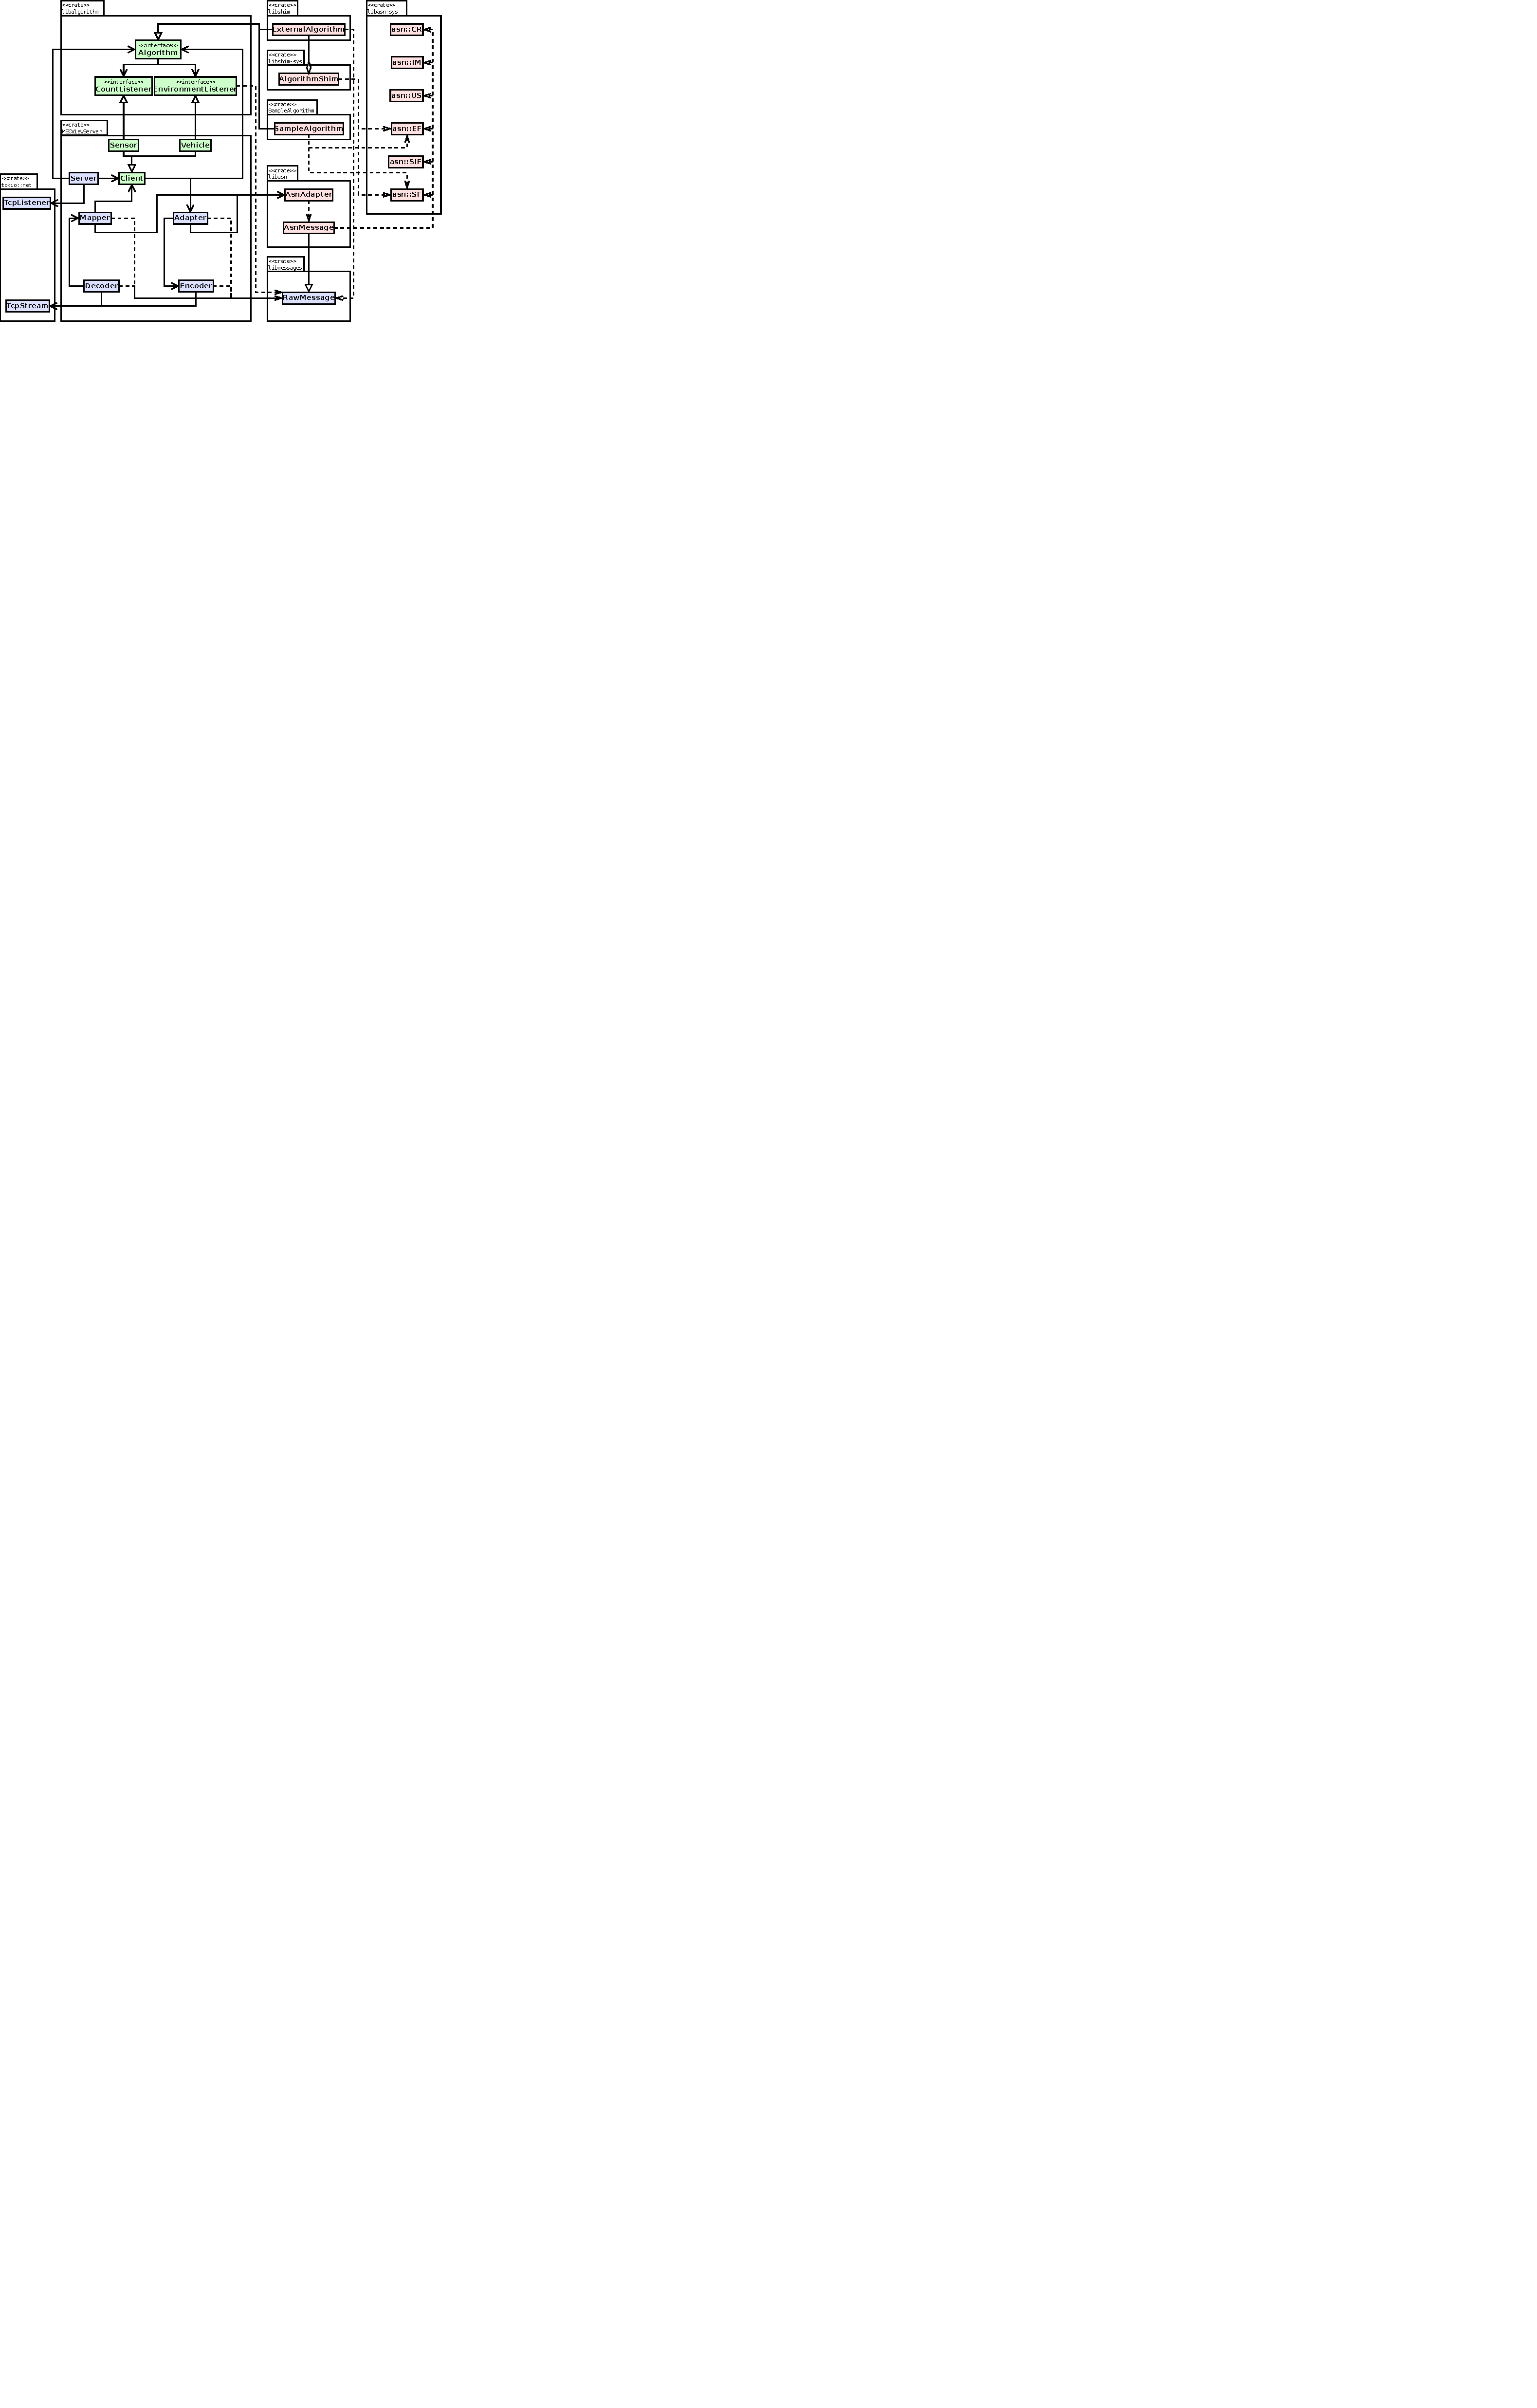
\includegraphics[width=3.3\textwidth]{dia/architecture_v2}
	\caption{Architekturentwurf}
	\label{draft:architecture_v2}
\end{figure}

Die \textit{Alogirhtm}-, \textit{CountListener}- und \textit{EnvironmentListener}-Schnittstelle wird in eine eigene Crate verschoben.
Die \textit{asn::Message} wird in \textit{AsnMessage} umbenannt und zusammen mit der \textit{AsnAdapter}-Klasse in die neue Crate \textit{libasn} verschoben.
Auch der \textit{SampleAlgorithm} wird in eine eigene Crate verschoben.
Zwei weiteren Crates binden den externen C++ Algorithmus ein: \textit{libshim-sys} um den C++ Code in Rust zugänglich zu machen (analog zu \textit{libasn-sys}) und \textit{libshim} für die Implementation der \textit{Algorithm}-Schnittstelle mittels Adaptercodes.

Die neuen Abhängigkeiten zwischen den Crates sind in \autoref{draft:architecture_v2_packages} zu sehen und entsprechen nun dem \enquote{Dependency Inversion Principle}. \todo{naja, teils}

\begin{figure}[H]
	\centering
	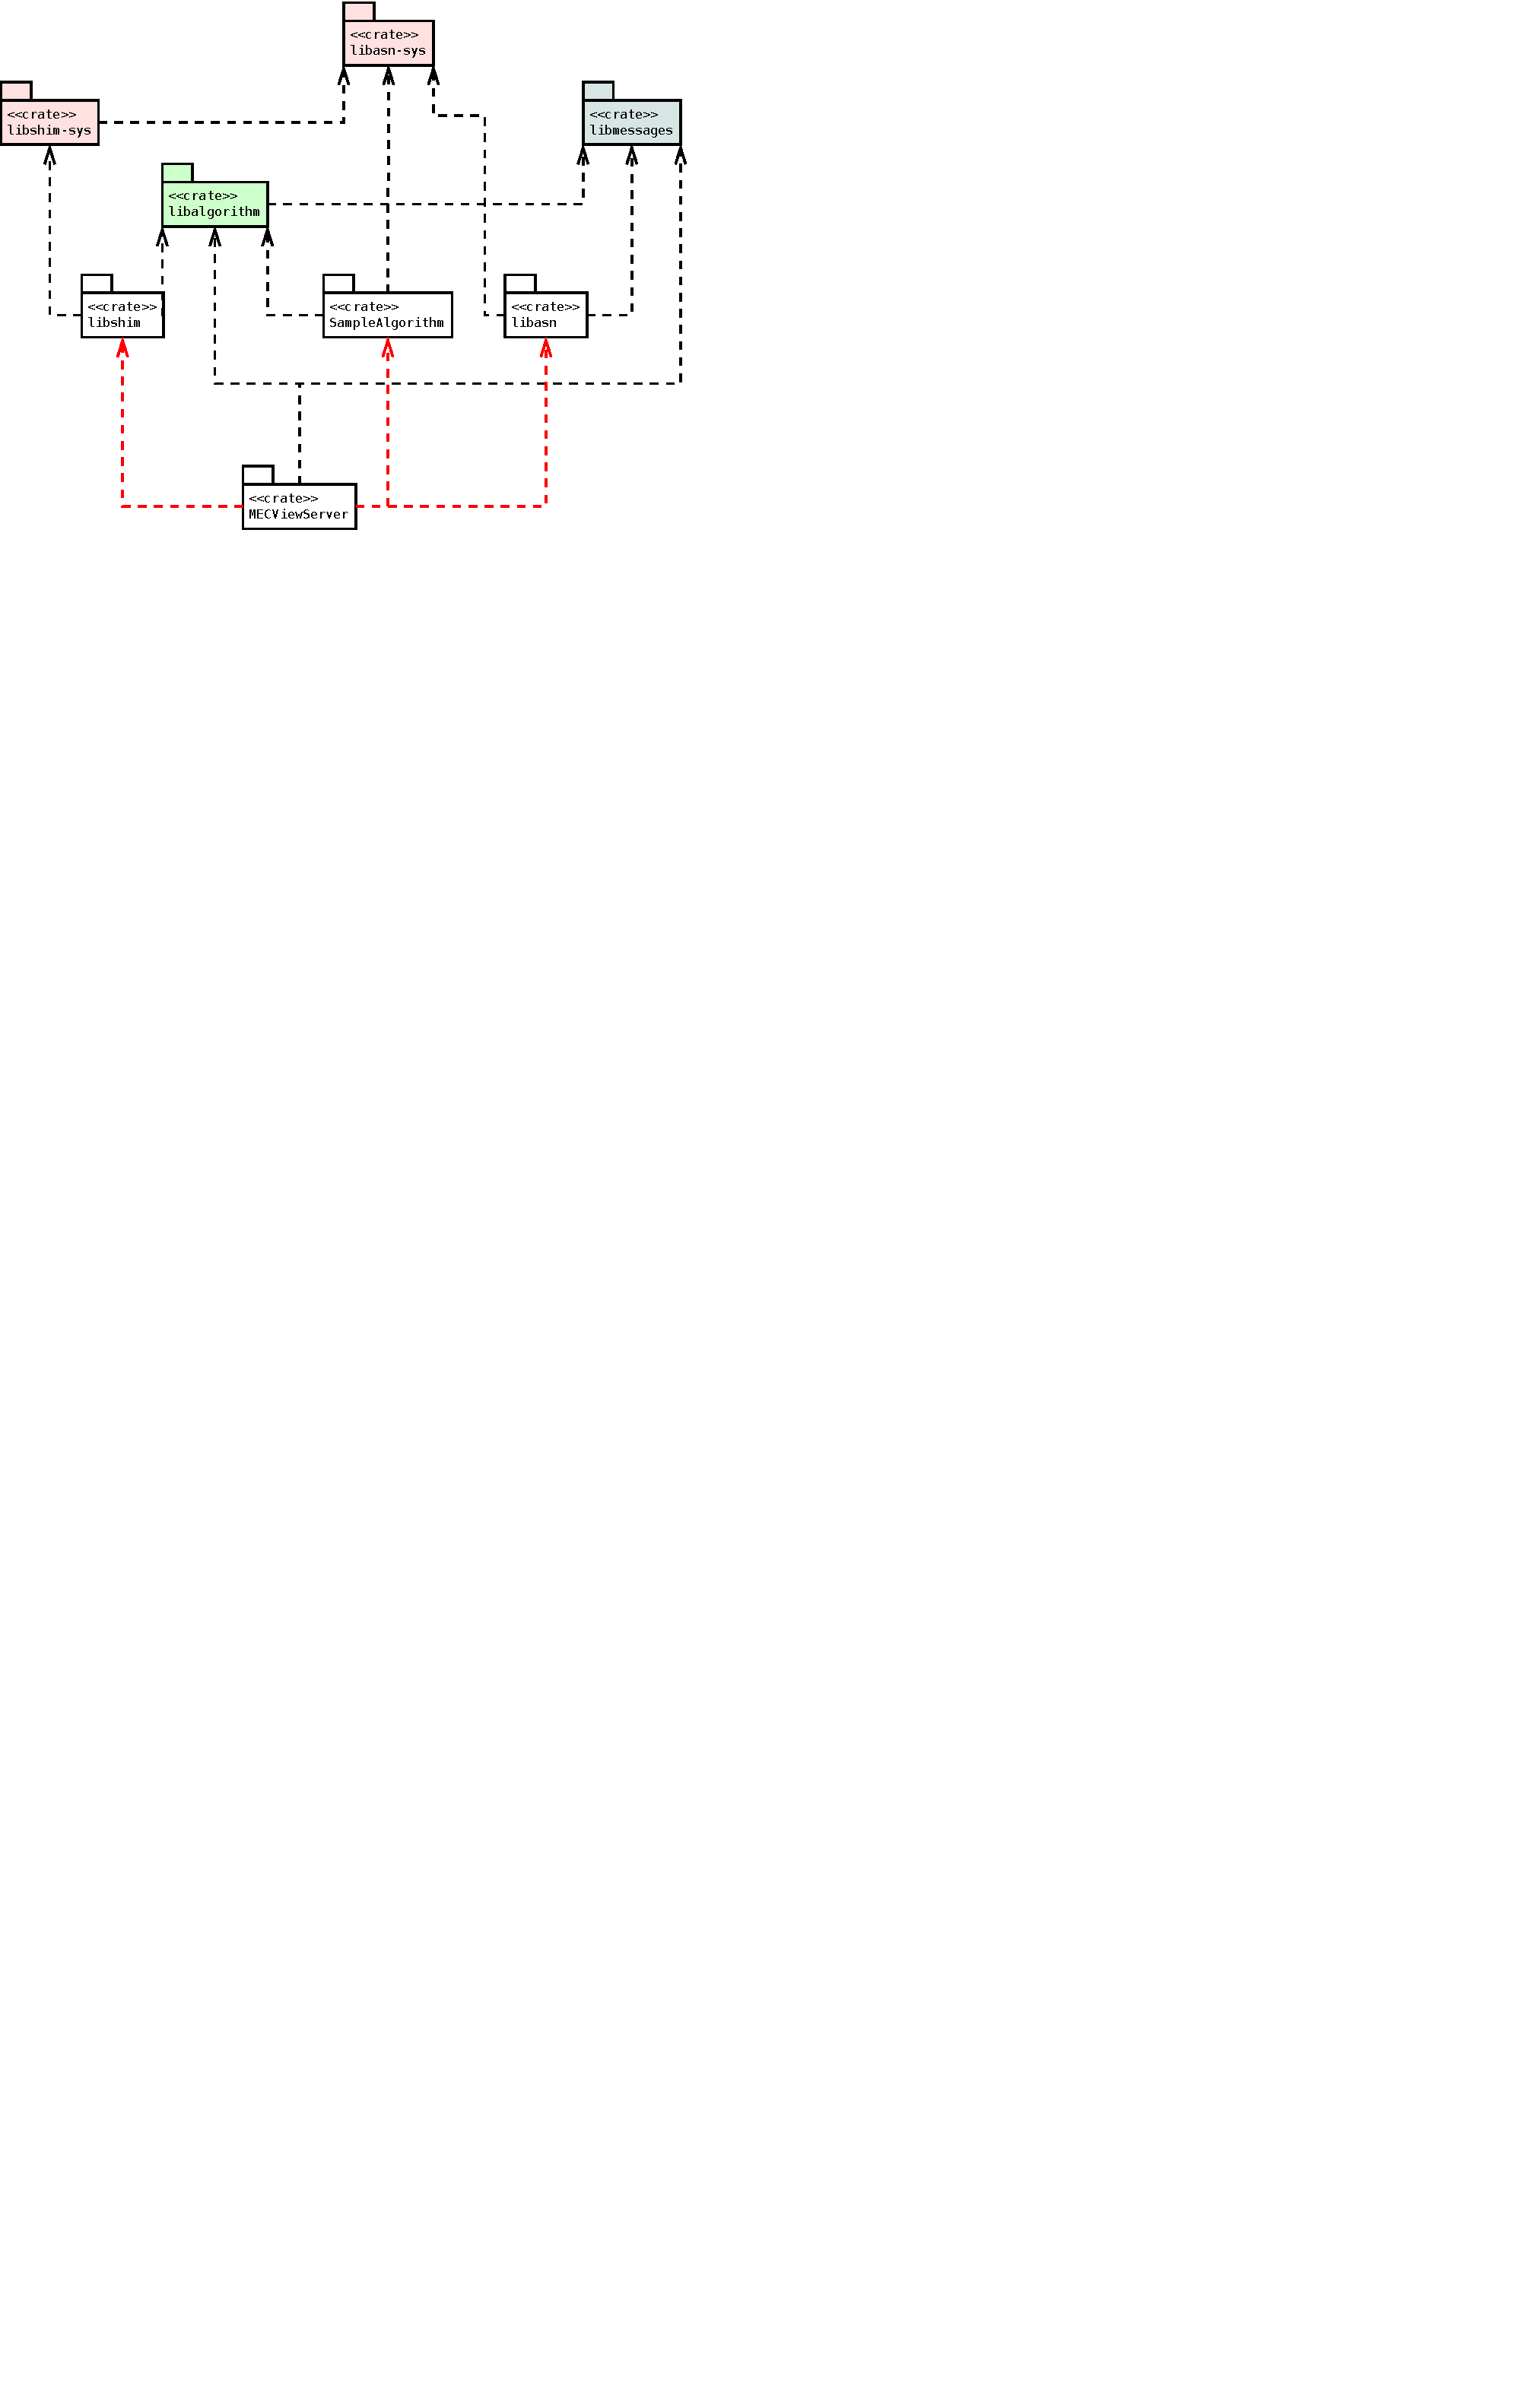
\includegraphics[width=1.9\textwidth]{dia/architecture_v2_packages}
	\caption{Architekturentwurf}
	\label{draft:architecture_v2_packages}
\end{figure}

Die roten Abhängigkeiten entstehen erst durch die Wahl einer Nachrichtentechnologie und des auszuführenden Algorithmus.
\todo{??}
Daher können sie als schwache Abhängigkeiten betrachtet werden.


\todo{.}
Die Einbindung des C++ Quellcodes ist, im Gegensatz zum C-Code der ASN.1 Nachrichten, deutlich schwieriger.
Die Abhängigkeiten zu den Datentypen der Standardbibliothek (siehe \autoref{class_dia:algorithm:cpp}) und die Klassenhierarchie macht einen Zugriff aus Rust deutlich komplizierter und würde eine manuelle Pflege der \textit{vtable} benötigen.
Deswegen ist eine andere Herangehensweise ausgewählt worden.
Weiterer C-Code soll den C++ Code über eine C-Datenstruktur und 5 Funktionen zugänglich machen \todo{Facade!} und eine Nutzung in Rust deutlich vereinfachen.
\todo{schwierig, bindgen nix c++}

\begin{figure}[H]
	\centering
	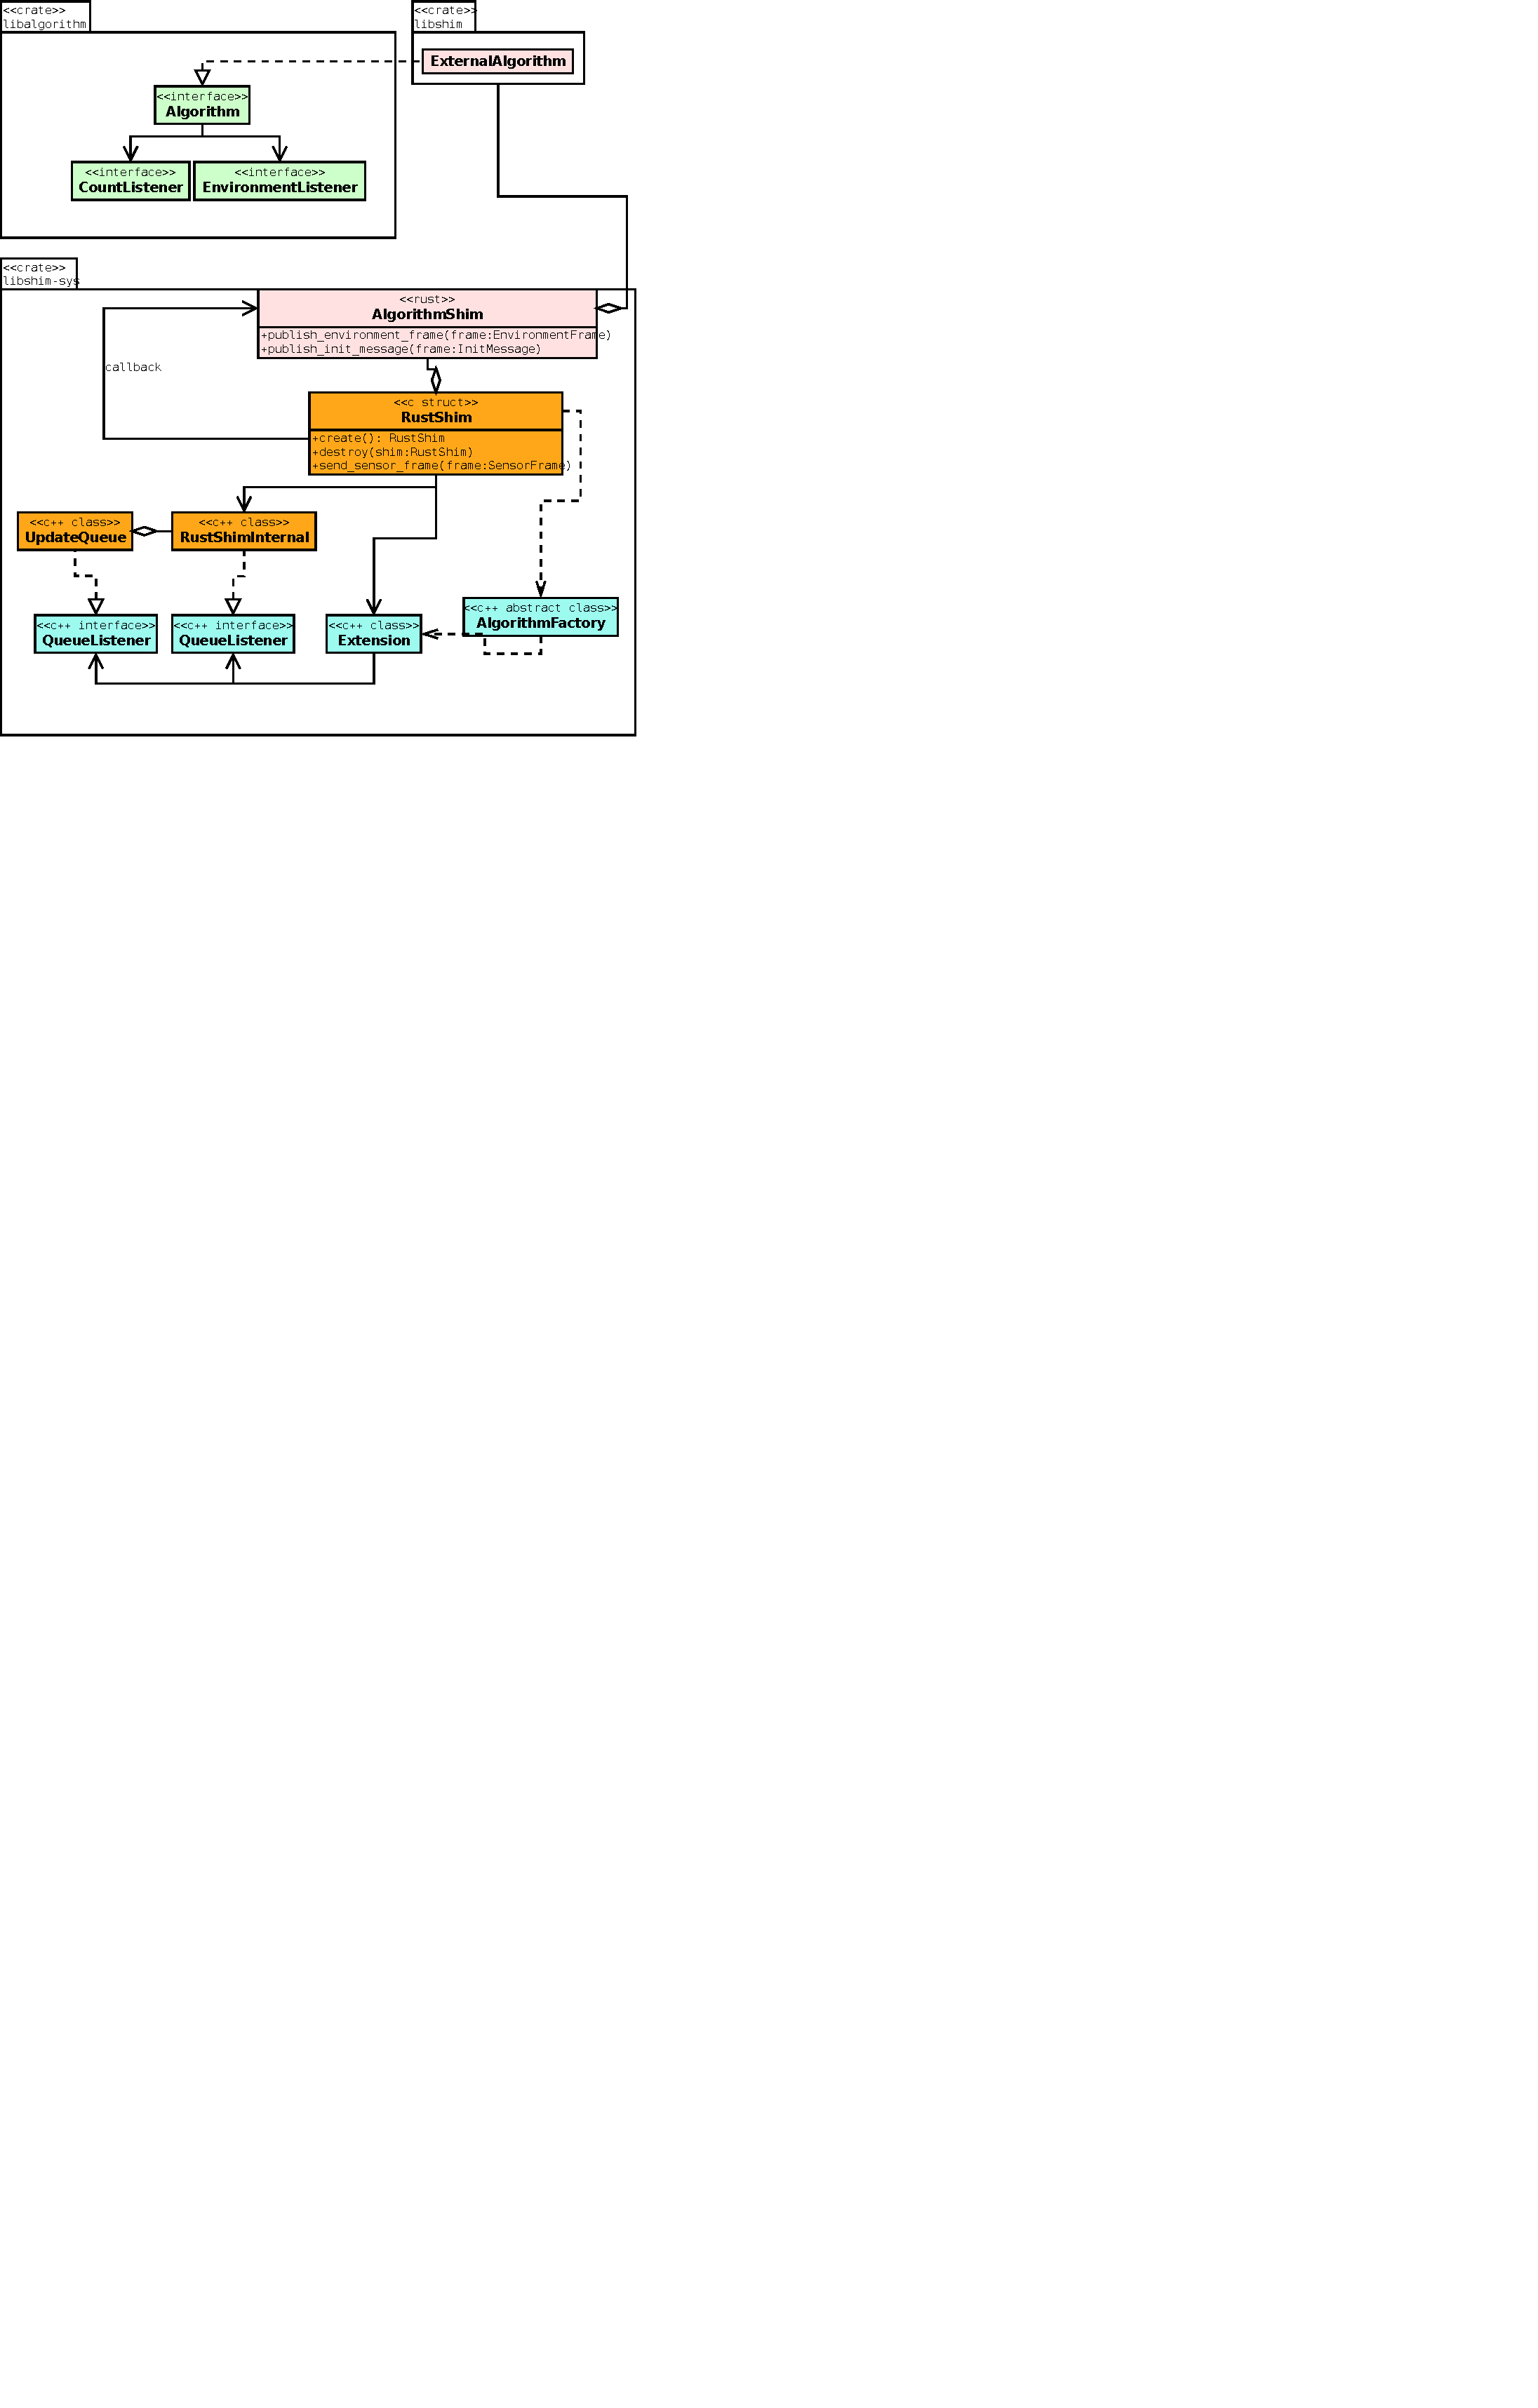
\includegraphics[width=2.5\textwidth]{dia/libshim}
	\caption{Detailansicht der Crate libshim-sys}
	\label{draft:libshim}
\end{figure}

\todo{zwei weitere hopps, komposition von AlgorithmShim verhindert dritten weiteren hopp}

\begin{landscape}
\vspace*{\fill}
\begin{figure}[H]
	\begin{tikzpicture}[scale=0.69, every node/.style={transform shape}]
	\begin{umlseqdiag} 
	\umlobject[x=-10,no ddots]{MEC-View-Server}
	%\umlmulti[x=-16,no ddots,class=Vehicle]{v}
	\umlobject[x=15,no ddots]{AlgorithmFactory}
	
	\begin{umlcreatecall}[x=-5,dt=5,class=ExternalAlgorithm]{MEC-View-Server}{a}
		\begin{umlcreatecall}[x=-1,dt=5,class=AlgorithmShim]{a}{ashim}
		
		\end{umlcreatecall}
	\end{umlcreatecall}
	%\umlcreatecall[x=-5,dt=5,class=ExternalAlgorithm]{MEC-View-Server}{a}
	%\umlcreatecall[x=-1,dt=5,class=AlgorithmShim]{a}{ashim}
	\umlcreatecall[x=3,dt=5,class=RustShim]{ashim}{rshim}
	\umlcreatecall[x=7,dt=5,class=RustShimInternal]{rshim}{i}
	\umlcreatecall[x=11,dt=5,class=UpdateQueue]{rshim}{q}
	
	\begin{umlcall}[op={<<static>> Create(e, q, config\_file)},return=a]{rshim}{AlgorithmFactory}
		\umlcreatecall[class=Extension,x=19]{AlgorithmFactory}{e}
	\end{umlcall}
	
	\umlmulti[x=-9,class=Sensor]{s}
	\begin{umlcall}[dt=2,op=update(SensorFrame), with return]{s}{a}
		\begin{umlcall}[op=publish\_sensor\_frame(SensorFrame), with return]{a}{ashim}
			\begin{umlcall}[op=Add(SensorFrame),with return]{ashim}{q}
				
			\end{umlcall}
		\end{umlcall}
	\end{umlcall}
	
	
	\begin{umlcall}[dt=17,op=Pop(),return=SensorFrame]{e}{q}
		
	\end{umlcall}
	
	
	\umlmulti[x=-12,y=-10,class=Vehicle]{v}
	\begin{umlcall}[op=,with return]{e}{i}
		\begin{umlcall}[op=,with return]{i}{rshim}
			\begin{umlcall}[op=,with return]{rshim}{ashim}
				\begin{umlcall}[op=,with return]{ashim}{a}
					\begin{umlcall}[op=Send(RawMessage),with return]{a}{v}
					\end{umlcall}
				\end{umlcall}
			\end{umlcall}
		\end{umlcall}
	\end{umlcall}
	
	\end{umlseqdiag} 
	\end{tikzpicture}
	\centering
	\caption{Instantiierung eines neuen C++ Algorithmus aus der Rust Implementation \todo{fix create calls}}
	\label{seq_dia:algorithm:cpp:binding}
\end{figure}
\vspace*{\fill}
\end{landscape}

%\todo{?? updated usecases}

%\todo{binary vs source code}

\clearpage
\section{Startparameter}

Alle in \autoref{requirements} genannten optionale Anforderungen für Startparameter sind erfolgreich umgesetzt worden.
Die Ausgabe in \autoref{help} zeigt alle möglichen Startparameter des Systems an.

\helpinclude
	{help}
	{Hilfsinformationen der Rust-Implementation mit allen möglichen Parametern}
	{sections/help.info}


In der folgenden Übersicht sind die Startparameter aus den Anforderungen, eine kurze Erklärung und ein Beispiel gelistet.

\newcommand{\proveReq}[3]{\textbf{Anforderung \reqNumberForLabel{#1}: \reqNameForLabel{#1}} \\ #2 \\ Beispiel: \monospaceinline{mecview_server #3}}

\begin{itemize}
	\item \proveReq{impl:arg:log}{
		Mit dem Startparameter \monospaceinline{-l <LEVEL>} (Kurzform) oder \monospaceinline{--log <LEVEL>} (Langform) kann einer der folgenden Level gesetzt werden: \monospaceinline{trace, debug, info, warn, err}.
	}{--log trace}
	
	\item \proveReq{impl:arg:interface}{
		Mit dem Startparameter \monospaceinline{-i <INTERFACE>} (Kurzform) oder \monospaceinline{--interface <INTERFACE>} (Langform) kann eine lokale Netzwerkadresse des Systems übergeben werden, auf der für eingehende TCP-Verbindungen gelauscht werden soll.
	}{-i 127.0.0.1}
	
	\item \proveReq{impl:arg:port}{
		Der Startparameter \monospaceinline{-p <NUMBER>} (Kurzform) und \monospaceinline{--port <NUMBER>} setzt den TCP-Port, den der Server verwendet, um auf neue Verbindungen zu lauschen.
	}{--port 4711}
	
	\item \proveReq{impl:arg:init_msg}{
		Mit dem Startparameter \monospaceinline{-v <PATH>} (Kurzform) oder \monospaceinline{--init-message <PATH>} (Langform) kann der Pfad zu einer in XML-Datei übergeben werden, aus der die zu verschickende \textit{InitMessage}-Nachricht geladen wird.
		}{--init-message scenario_5086.xml}
		
	\item \proveReq{impl:arg:env_frame}{
		Mit dem Startparameter \monospaceinline{-e <PATH>} (Kurzform) oder \monospaceinline{--environment-frame <PATH>} (Langform) kann der Pfad zu einer in XML-Datei übergeben werden, aus der die zu verschickende \textit{EnvironmentFrame}-Nachricht geladen wird.
	}{-e Kreuzung_2.xml}
	
	\item \proveReq{impl:arg:alg_json}{
		Der Startparameter \monospaceinline{-a <PATH>} (Kurzform) und \monospaceinline{--algorithm <PATH>} setzt den Pfad, der dem externen C++ Algorithmus bei der Initialisierung übergeben wird.
		Wenn der \enquote{Dummy}-Algorithmus verwendet wird, wird dieser Parameter ignoriert.
		}{-a latency_measurement.json}
\end{itemize}


\section{?? Bindgen für ASN}

\label{impl:issue:ffi}
\todo{schnell problem: kein asn->rs compiler, c bindings aufwending -> autogen via bindgen}

\todo{link issues fixed in commit d5d694c}

\todo{impl Drop / free structs, important but do not overengineer}

\section{...}

\todo{bzgl coverage viele tests für encodieren / decodieren, server instanz nicht getestet weil nur mit tokio verdrahtet... schwierig zu testen}


\todo{tdd schwierig weil viel integration mit framework / async, schnell wird daraus integrationstest(?, unerwünscht)}

\todo{rust-clippy: https://github.com/rust-lang-nursery/rust-clippy}


\section{Strategien für Performance}

\todo{\enquote{bypass} via RawMessage for algorithm->many vehicles}





\todo{diagramm: jede future ein eigenes "paket", queues dazwischen für kommunikation}

\todo{catch panic? mention how in \autoref{rust:no_null}}

\todo{SRP, impl Object separat from impl CommandProcessor for Object, testability?}




\section{libmessages make unsafe libmessages-sys safe}
	
\subsection{Vorgehen, bindgen tests, C/unsafe/wrapper -> nach sicher ->  architektur entwickeln}
	

	
\section{Unerwartete Schwierigkeiten}
	
	\todo{Trailing zeroes issue, commit a02496d + tagged, libmessages/src/asn.rs:17 bzw :31 bzw :32 Ok((result.encoded as usize + 7) / 8}
	
	\todo{unterschiedlicher Heap libc / rust --> Rust Heap wird von Rust aufgeräumt, libc von libc... or deadlock}
	
	\todo{jenkins clippy nightly often broken}
	
	\todo{RawMessage<T> machts leben schwer}
	
\subsection{Schwierigkeit: Heap nicht gleich Heap}

\todo{deadlock im heap allokieren, rust heap muss von rust aufgeräumt werden, libc von libc, asn+c++-alg -> libc}


\section{Valgrind: Race Conditions all over the place}

\section{Mocks für TDD}
